\documentclass[letterpaper,twocolumn,12pt]{article}
\usepackage[T1]{fontenc}
\usepackage[margin=1in]{geometry}
\usepackage{graphicx}
\usepackage{ulem}

\pagestyle{empty}
\setlength{\columnsep}{2em}
\title{A Survey of Hardware Multithreading}
\author{Sol Boucher \\ Carnegie Mellon University \\ sboucher@cs.cmu.edu}
\date{}

\begin{document}
\maketitle
\thispagestyle{empty}

\subsection*{Abstract}
I'm just going to assume you already read the title.
We chose a needle as our hardware threading platform because the author had a rip in his pants.
\sout{More concretely,} you'll have to read the paper for details; after all, this is just the abstract.

\section{Introduction}
This paper describes our first-hand experiences with needle threading in hardware.
This paper is organized as follows:\@
on second thought, why don't you just skim the section titles like a normal reader and work that out on your own?

\section{Test Environment}
We remind the reader that we were suffering from a pair of ripped pants at the time of writing.
We hadn't expected the pair of pants in question to be ripped, and this misprediction led to a stall in our laundry pipeline.
This resulted in a phenomenon we'll refer to as \textit{cold legs}, so we began eyeing our bed as a potential location to continue the research.
In the interest of full disclosure, there are a few admissions we should make about this test bed:
\pagebreak
\begin{itemize}
\item It could have been better made.
\item We briefly attempted to remedy this issue, but ultimately concluded that this is a hard problem.
\item We conjecture that making the bed is actually an unimportant step, as our next step was to crawl in.
\item For months now, we've been operating under the assumption that this conjecture is correct; however, it would be good to have rigorous proof.
\end{itemize}

\section{Design}
The core idea of multithreading is, of course, to improve efficiency by performing parallel work.
To begin our investigation, we attached multiple threads to the same needle, as shown in Figure~\ref{fig:thread}.
While this sounds like a simple process, care must be taken to ensure that each individual thread is attached directly to the needle, as tying them end-to-end does not increase parallelism.

\begin{figure}[h]
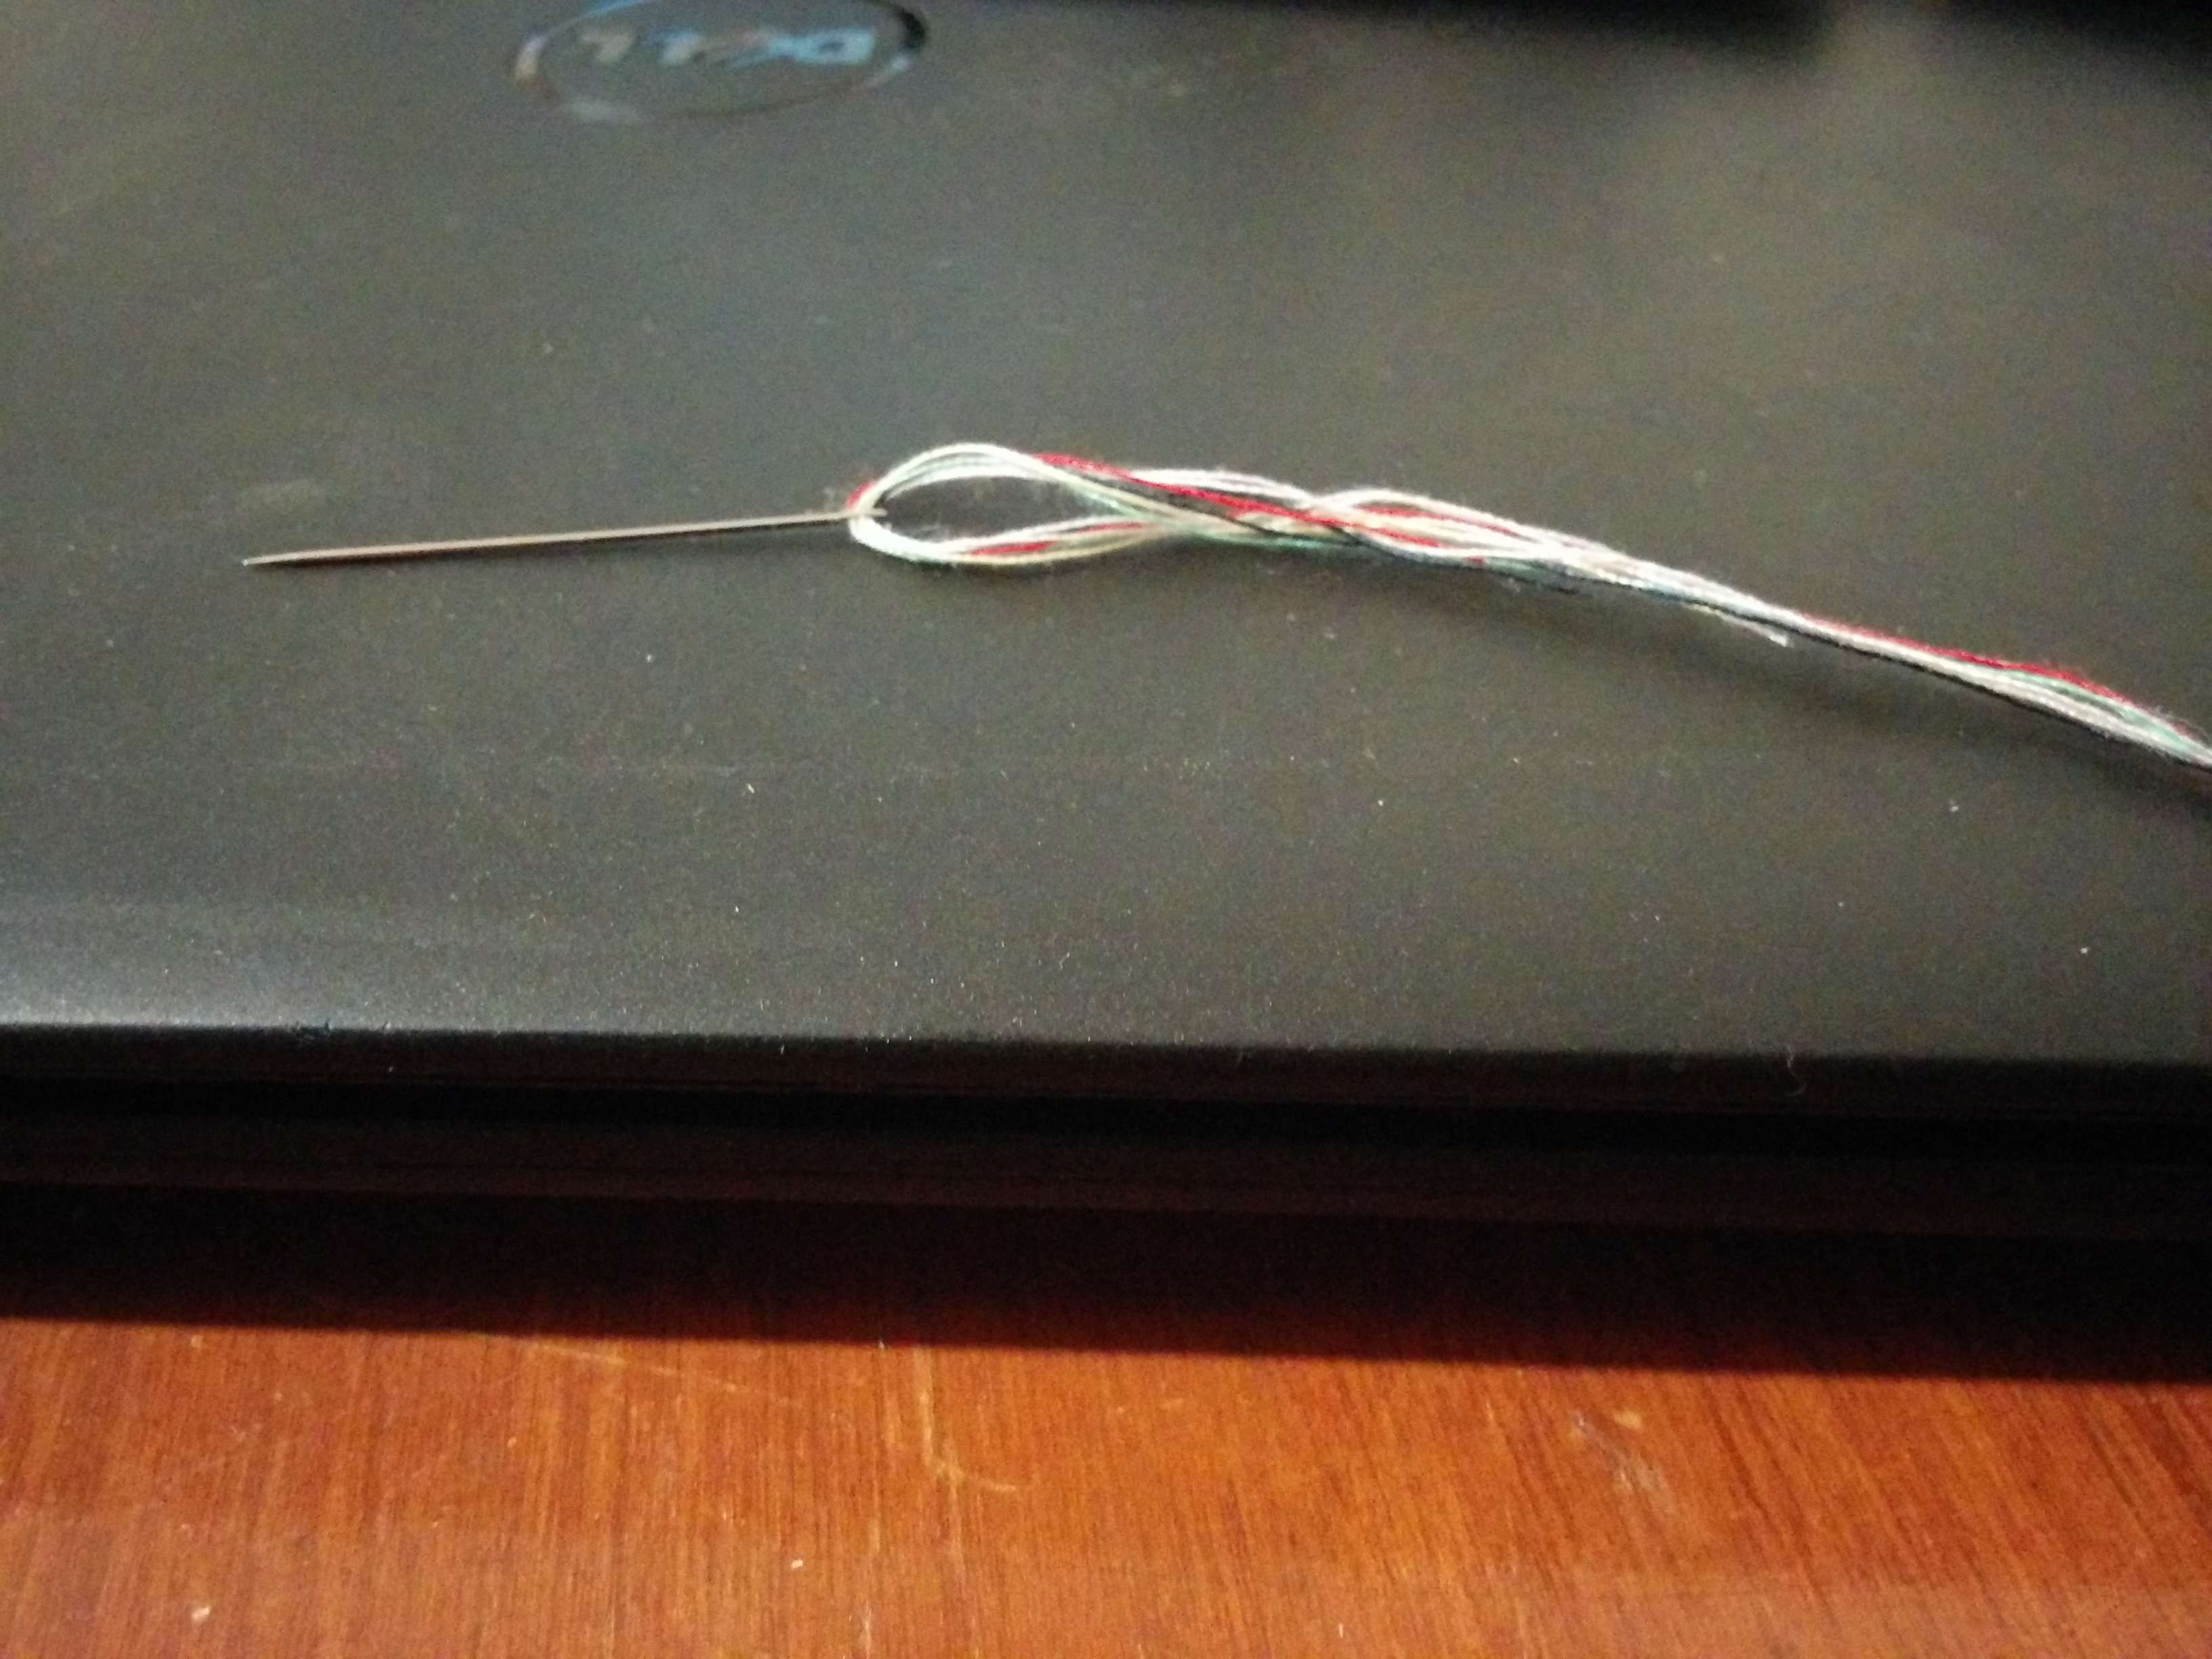
\includegraphics[width=\columnwidth]{thread}
\caption{Multithreading}
\label{fig:thread}
\end{figure}

\section{SMT}
Before tying the threads to the needle, we discovered that they were asymmetrically threaded.
We tried to balance them to achieve the desired symmetry, but this turned out to be imprecise when attempted by hand.
We attempted to employ an SMT solver, but it seemed confused.
Perhaps we should have paid more to hire one with better SAT scores, as we've been told that such solvers have quickly reported NP-complete (``No Problem, done'') when faced with similar challenges.

\section{Parallelism}
\label{sec:parallelism}
To further motivate multithreading, we observe that the number of threads used in the test fabric is proportional to its resultant tensile strength.
By Amdahl's law, increasing the parallelism decreases the time taken to achieve a given tensile strength.
Needle-less to say, this trend would continue if our needle could accommodate more threads.
As it is, we were only able to test at limited scale, but we posit that better hardware would allow us to quickly handle the Big Rip.

\section{Coherency}
In our experience, even the amount of parallelism achievable on our platform is difficult to manage.
We struggled repeatedly as the, um, data became stuck in our KNOT gates.
It wasn't until we dropped the needle, though, that the true extent of our catch coherency issues became apparent.

\section{Future Work}
We'd like to extend this work to test on platforms other than beds (e.g.\@ haystacks).
Although it seemed inappropriate for the repair in question, an investigation into threads that collect user input is sorely needed, not least because we have a bunch of spare buttons lying around.
As more threads become involved, managing concurrency becomes increasingly critical; therefore, an investigation into the threading of eyebrows, locks, and other synchronization mechanisms is also in order.

\section{Conclusion}
As foreshadowed in Section~\ref{sec:parallelism}, we suggest that future hardware include a larger loop thing so the needle can accommodate more threads.
That said, the limited amount of parallelism we were able to achieve resulted in a pair of pants that allowed us to leave the test bed but not the house.
We take the fact that we couldn't wear them in public as an indication that the problem is embarrassingly parallel.

\section*{Acknowledgements}
We are grateful to the Lord for being our shepherd.
Without Her assistance, the market economy would never have been able to capture enough sheep to supply the many threads required by our system.

\section*{References}
``For the absence of a bibliography\footnote{or citation for this quotation} I offer neither explanation nor apology.''

\end{document}
